\section{Cơ sở lý thuyết}
\subsection{Phương pháp áp dụng - KGAT}
Phương pháp tiếp cận gần đây - KGAT: Knowledge Graph Attention Network for Recommendation

Bài báo đề xuất một phương pháp để cải thiện độ chính xác, đa dạng và khả năng giải thích của hệ thống gợi ý, cần phải xem xét thêm thông tin bổ sung thay vì chỉ dựa vào tương tác người dùng-sản phẩm. Thường thì các phương pháp truyền thống như học máy không đủ để nắm bắt các mối quan hệ phức tạp giữa các mục, từ đó cho ra kết quả dự đoán kết quả không được cao. Trong nghiên cứu này, nhóm tác giả sử dụng đồ thị tri thức (Knowledge Graph) để liên kết các mục với thuộc tính của chúng, cho rằng các quan hệ bậc cao là chìa khóa cho việc gợi ý hiệu quả. Tổng quan phương pháp này được gọi là Knowledge Graph Attention Network for Recommendation (KGAT) [3], mô hình hóa rõ ràng các kết nối bậc cao và sử dụng cơ chế chú ý để đánh giá tầm quan trọng của các liên kết. Kết quả thực nghiệm cho thấy KGAT vượt trội hơn các phương pháp tiên tiến hiện có và cung cấp khả năng giải thích tốt hơn.

KGAT là một trong những hệ thống đề xuất tập trung nhiều hơn về những thông tin ẩn về người dùng. Bằng cách kết hợp nhúng nhiều trường thông tin ẩn vào mô hình, nhóm tác giả đã tạo được một mô hình không chỉ hiểu về những thông tin rõ ràng đã có của người dùng mà còn các tương tác ẩn giữa người dùng với các đối tượng đó.

\subsubsection{Các kiến thức cần nắm}
Bài báo KGAT đề xuất một phương pháp xử lý dữ liệu tốt hơn bằng cách tận dụng trường thông tin bổ sung (Item side information) để tăng hiệu suất của mô hình.

Giải quyết bài toán đề xuất với cách tiếp cận là tạo ra một mô hình có mối quan hệ bậc cao rõ ràng giữa các trường thông tin và toàn diện với cách xử lý của một mạng thần kinh đồ thị (Graph Neural Network [8] [9] – GNN).

Tiến hành mở rộng và so sánh với các phương pháp kinh điển trước đó để chứng minh được hiệu suất rõ ràng của mô hình.

Về tổng quát, có thể thấy KGAT tập trung phát triển và cải thiện các kĩ thuật xử lý dữ liệu dựa trên GNN. Vậy GNN là gì? Cốt lõi của GNN là gì? Đáp án của những câu hỏi trên nằm ở một câu trả lời duy nhất, đó là đồ thị tri thức (Knowledge Graph - KG). KG có thể được hiểu là một mạng phức tạp liên kết các thực thể - chẳng hạn như giữa người dùng (users), vật phẩm (items) và các đặc trưng (features) của chúng thông qua mối quan hệ phức tạp của chúng.

\begin{figure}[h]
    \centering
    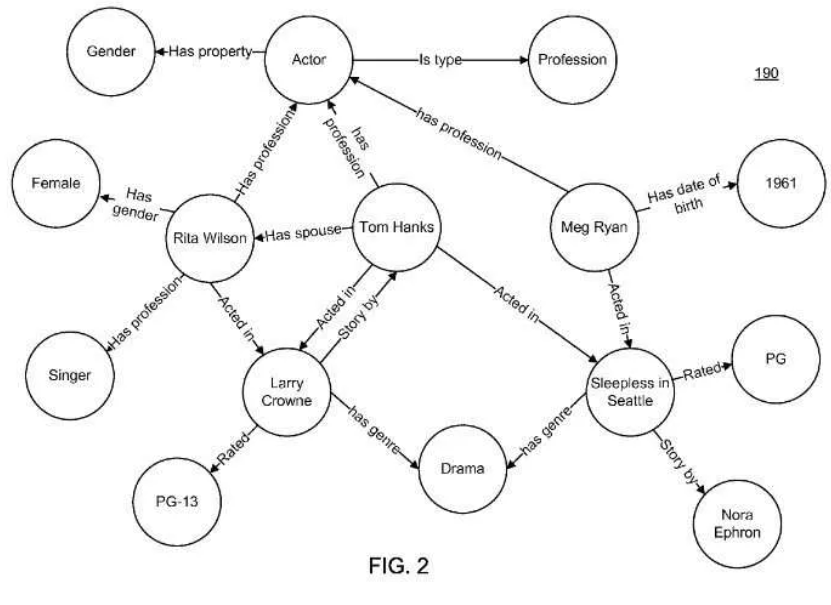
\includegraphics[width=0.8\textwidth]{figures/64.png}
    \caption{Biểu đồ tri thức KG trong thực tế}
    \label{fig:kg_example}
\end{figure}

Thường thì, các thành phần cấu tạo nên một KG sẽ bao gồm:
\begin{itemize}
    \item Nút: đại diện cho các thực thể (ví dụ: người dùng, sản phẩm, danh mục, …)
    \item Cạnh: mô tả mối quan hệ của các nút (ví dụ: đã mua, đã xem, …. Và ngược lại)
\end{itemize}

Có thể thấy đây là một kiến trúc mạng linh hoạt có nhiều lớp thông tin có thể được bổ sung và tích hợp với nhau, điều này cho phép một mạng KG có thể hiểu được toàn diện về ngữ cảnh và môi trường của người dùng nếu được tổ chức tốt.

\subsubsection{Tổng quan về KGAT}
Mô hình KGAT sử dụng thông tin bổ sung để xây dựng một biểu đồ tri thức nhằm nắm bắt mối quan hệ giữa người dùng, các mục (items) và các tương tác người dùng (user interaction) với nhau. Mô hình KGAT sử dụng cơ chế học chú ý (Attention Mechanism) với đồ thị nhằm cho phép mô hình có thể hiểu được tầm quan trọng về sự khác nhau giữa các vật phẩm và những đặc trưng của chúng. Điểm khác biệt giữa mô hình KGAT so với các mô hình trước đây là nó được thiết kế với sự thay đổi nhằm làm phong phú thêm về sự hiểu biết của mô hình về hành vi và sở thích của người dùng. Điều này dẫn đến những dự đoán không chỉ dựa trên những thuộc tính của các mục (items) mà còn được định hình dự trên đặc điểm của từng người dùng, giúp cải thiện đáng kể độ phù hợp và liên quan giữa các mục được mô hình đề xuất.

\begin{figure}[h]
    \centering
    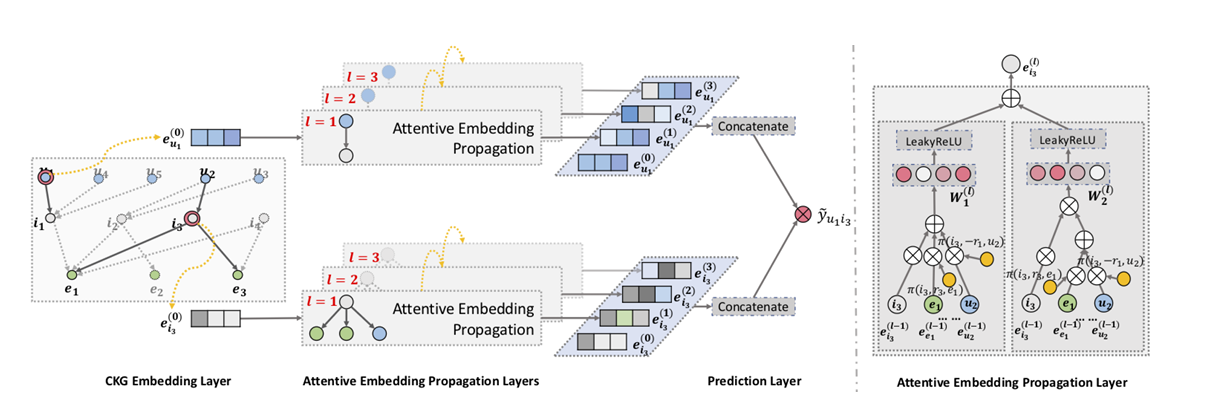
\includegraphics[width=0.8\textwidth]{figures/65.png}
    \caption{Kiến trúc tổng quan mô hình khuyến nghị học sâu KGAT}
    \label{fig:kgat_model}
\end{figure}

\subsubsection{Các kĩ thuật sử dụng của KGAT}
\paragraph{Embedding layer.}
Về mặt lý thuyết, tác giả tạo một collaborative knowledge graph – CKG. CKG là sự kết hợp giữa một KG và một user-item bipartile graph. CKG có thể được hiểu là một dạng mở rộng của một KG, trong đó thông tin không chỉ đến từ thông tin của User và Item mà còn đến từ các thông tin bổ trợ khác (ở hình sau là các Entities). Mục tiêu của một CKG là sử dụng được thông tin phong phú từ nhiều nguồn để cải thiện độ chính xác và tăng khả năng dự đoán của mô hình.

\begin{figure}[h]
    \centering
    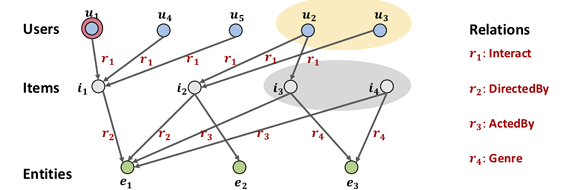
\includegraphics[width=0.8\textwidth]{figures/66.png}
    \caption{Một CKG biểu diễn liên kết cho các loại thực thể}
    \label{fig:ckg_example}
\end{figure}

Điểm hay của KGAT là khai thác được các quan hệ bậc cao trong CKG, ví dụ như các kết nối dài hạn sau:
\begin{itemize}
    \item u1  r1→  i1  -r2→  e1  r2→  i2  -r1→  \{u2,  u3\}
    \item u1  r1→  i1  -r2→  e1  r3→ \{i3,  i4\}
\end{itemize}

Về cách thức thực hiện, embedding layer tham số hóa các thực thể và quan hệ dưới dạng các vectors trong khi vẫn bảo toàn cấu trúc đồ thị. Trong bài báo, nhóm tác giả sử dụng TransR [10] để tham số hóa các thực thể và mối quan hệ trong CKG thành các biểu diễn vector, xem xét sự biểu diễn của chúng với kết nối trực tiếp của mỗi bộ ba phần tử (h, r, t):

\begin{figure}[h]
    \centering
    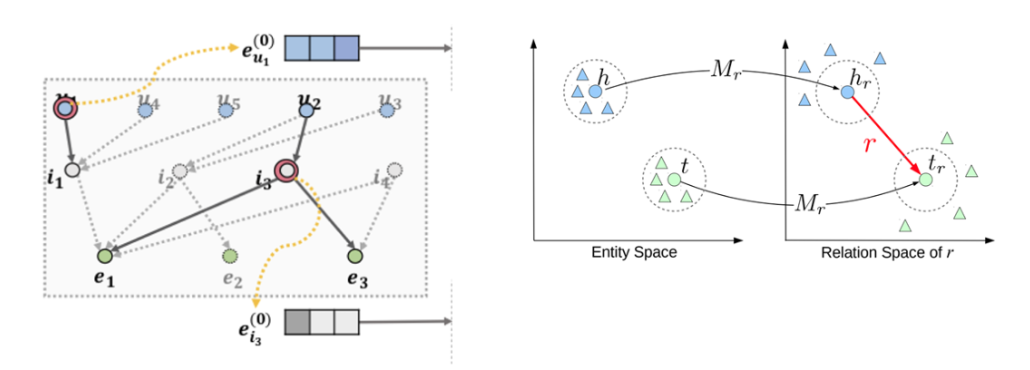
\includegraphics[width=0.8\textwidth]{figures/67.png}
    \caption{Cơ chế embeddings (bên trái) và TranR (bên phải) trong KGAT}
    \label{fig:embedding_process}
\end{figure}

\paragraph{Attentive Embedding propagation layers.}
Về lý thuyết, đây được xem như giai đoạn biểu diễn mỗi nút dưới dạng một vector bằng cấu trúc bảo toàn cấu trúc của CKG, đệ quy lan truyền để truyền các lớp nhúng học được từ các nút lân cận để cập nhật biểu diễn cho nó, sử dụng cơ chế học có chú ý (Attention) để học chi tiết từng trọng số cho các nút lân cận trong quá trình lan truyền.

\begin{figure}[h]
    \centering
    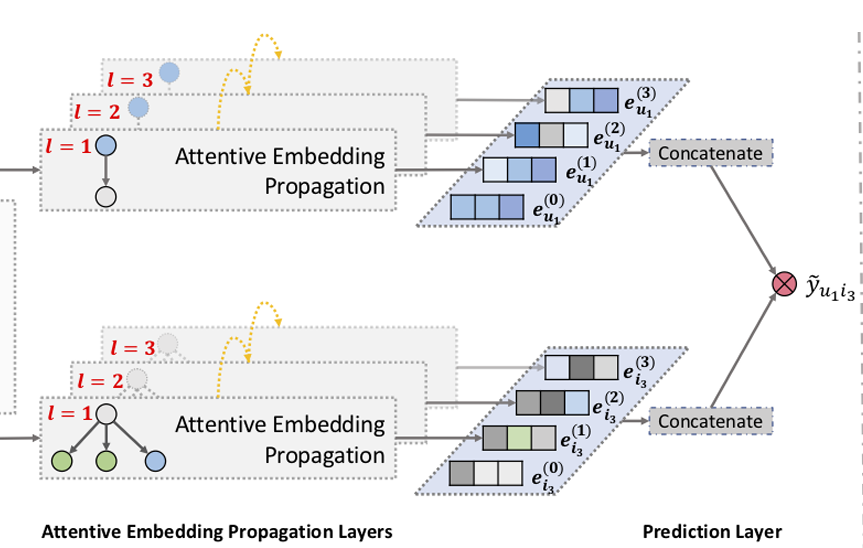
\includegraphics[width=0.8\textwidth]{figures/68.png}
    \caption{Cơ chế Attention và cơ chế truyền thông tin giữa các lớp}
    \label{fig:attention_process}
\end{figure}

Cách tiếp cận có hệ thống này biến mô hình KGAT thành một hệ thống kết hợp nắm bắt cả các thông tin items trực tiếp của người dùng và bối cảnh rộng hơn của các tùy chọn đó, tạo ra một hệ thống đề xuất rõ ràng hơn có khả năng mang được nhiều thông tin để dự đoán hơn.

\paragraph{Model prediction.}
Sau khi thực hiện lan truyền thông tin qua L lớp, ta thu được nhiều đại diện của người dùng node u, bao gồm: \{eu(1), …, euL\}; tương tự với sản phẩm node i, ta cũng thu được ei1,…,eiL. Tiếp đến, ta sẽ ghép nối embedding ban đầu với các embeddings mới thu được theo công thức sau:
\[
eu* = eu(0) || … || eu(L), \quad ei* = ei(0) || … || ei(L)
\]
Cuối cùng, điểm số phù hợp (matching score) giữa người dùng và sản phẩm sẽ được tính bằng inner product:
\[
yu,i = eu*T e i*
\]

Về cách thức tối ưu, KGAT sử dụng loss function chính xác đối với thói quen tương tác người dùng.

\subsection{Phương pháp khác}
\subsubsection{Content-based Filtering}
\textbf{Giới thiệu sơ thuật toán}\\
Ở đề tài này, ta sử dụng mô hình \textbf{Content-based Filtering} dựa trên các đặc điểm của khóa học để đề xuất những khóa học có nội dung tương tự cho người dùng, dựa trên sở thích và lịch sử học tập của họ. Ví dụ, nếu người dùng đã tham gia các khóa học thuộc một chủ đề nhất định, hệ thống sẽ đề xuất các khóa học có chủ đề tương tự.\\
\\
Để hiểu rõ hơn về khái niệm của mô hình này, ta sẽ đồng thời tìm hiểu về mô hình \textbf{Collaborative Filtering} để đối chiếu và đưa ra các điểm khác biệt giữa chúng.\\
\\
Trước hết,  \textbf{Content-based Filtering} và \textbf{Collaborative Filtering} là hai phương pháp khuyến nghị phổ biến, và điểm khác nhau giữa chúng là cách sử dụng dữ liệu và cách xây dựng đề xuất. Dưới đây là các điểm khác biệt chính:\\
\textbf{a. Cơ sở dữ liệu sử dụng}
\begin{itemize}
    \item \textbf{Content-based Filtering:} Dựa trên các đặc điểm và nội dung của mục tiêu cần khuyến nghị (items), chẳng hạn như mô tả khóa học, chủ đề, hay lĩnh vực học tập. Hệ thống đề xuất những khóa học có nội dung tương tự với các khóa học mà người dùng đã tham gia trước đó. Các thuộc tính của khóa học hoặc mục tiêu sẽ được mã hóa dưới dạng vector đặc trưng, và hệ thống sử dụng các vector này để tìm ra các khóa học tương tự.
    \item \textbf{Collaborative Filtering:} Dựa trên sở thích và hành vi của người dùng như xếp hạng, đánh giá, hoặc lượt xem. Thay vì dựa vào nội dung của các mục tiêu, Collaborative Filtering sử dụng thông tin về cách người dùng tương tác với các mục tiêu, và dựa vào đó để đưa ra các gợi ý dựa trên sự tương đồng giữa người dùng hoặc giữa các khóa học.
\end{itemize}
\textbf{b. Phương pháp tiếp cận}
\begin{itemize}
    \item \textbf{Content-based Filtering:} Dựa vào hồ sơ sở thích của từng người dùng để cá nhân hóa đề xuất. Nếu một người dùng đã xem nhiều khóa học thuộc lĩnh vực A, hệ thống sẽ đề xuất các khóa học khác trong cùng lĩnh vực, dựa trên các đặc điểm giống nhau.
    \item \textbf{Collaborative Filtering:} Có hai hướng tiếp cận chính:
\end{itemize}
\begin{itemize}
    \item
    \begin{itemize}
        \item User-based Collaborative Filtering: Đề xuất dựa trên những người dùng có sở thích tương tự. Ví dụ, nếu người dùng A và B có cùng sở thích trong một số khóa học, hệ thống có thể gợi ý cho A các khóa học mà B đã tham gia, và ngược lại.
        \item Item-based Collaborative Filtering: Đề xuất dựa trên các khóa học tương tự mà nhiều người dùng cùng yêu thích. Ví dụ, nếu nhiều người dùng học cả khóa X và Y, hệ thống sẽ đề xuất khóa Y cho những người dùng chỉ mới học khóa X.
    \end{itemize}
\end{itemize}
\textbf{c. Yêu cầu về dữ liệu}
\begin{itemize}
    \item \textbf{Content-based Filtering:} Cần có thông tin chi tiết và mô tả về từng mục tiêu (khóa học, phim, sản phẩm), chẳng hạn như từ khóa, chủ đề, hoặc bất kỳ đặc điểm nào liên quan đến nội dung của mục tiêu. Cách tiếp cận này ít phụ thuộc vào dữ liệu người dùng nhưng yêu cầu dữ liệu chất lượng về nội dung.
    \item \textbf{Collaborative Filtering:} Phụ thuộc vào dữ liệu về tương tác của người dùng, nên yêu cầu lượng người dùng lớn và tương tác phong phú. Phương pháp này có thể gặp khó khăn khi dữ liệu thưa (khi người dùng mới hoặc khóa học mới chưa có nhiều tương tác), dẫn đến vấn đề cold-start.
\end{itemize}
\textbf{d. Ưu và nhược điểm}
\begin{itemize}
    \item \textbf{Content-based Filtering:}
    \begin{itemize}
        \item Ưu điểm: Có thể gợi ý khóa học ngay cả khi người dùng không có nhiều tương tác; phù hợp cho trường hợp cold-start ở mức độ nhất định.
        \item Nhược điểm: Dễ dẫn đến sự lặp lại và thiếu đa dạng vì chỉ đề xuất nội dung tương tự; không dễ phát hiện những sở thích tiềm ẩn ngoài những gì người dùng đã học.
    \end{itemize}
    \item \textbf{Collaborative Filtering:}
    \begin{itemize}
        \item Ưu điểm: Khả năng khám phá các khóa học ngoài sở thích hiện tại của người dùng; thường đưa ra các gợi ý đa dạng hơn vì dựa trên hành vi tập thể.
        \item Nhược điểm: Không hoạt động hiệu quả trong tình huống cold-start; cần lượng dữ liệu lớn về tương tác giữa người dùng và mục tiêu để có hiệu quả cao.
    \end{itemize}
\end{itemize}

\subsubsection{Matrix Factorization - Bayesian Personalized Ranking}


Bayesian Personalized Ranking (BPR) là một phương pháp học máy được thiết kế đặc
biệt để cải thiện hệ thống gợi ý, đặc biệt là trong bối cảnh dữ liệu phản hồi
ngầm (implicit feedback) như lượt xem, lượt mua, hay lượt thích.

Khi kết hợp với Matrix Factorization (MF), BPR đã chứng minh hiệu quả vượt trội
trong việc cá nhân hóa đề xuất sản phẩm cho người dùng.Trong bối cảnh BPR, dữ
liệu thường là dạng phản hồi ngầm, tức là chỉ biết được các tương tác tích cực
(ví dụ: người dùng đã mua hoặc xem sản phẩm nào đó) màk hông có thông tin về
các tương tác tiêu cực. BPR giả định rằng những mục khôngđược tương tác là
không được ưu tiên hoặc ít được ưu tiên hơn so với những mục đã được tương tác.

Matrix Factorization là kỹ thuật phổ biến để phân rã ma trận người dùng mục
thành các ma trận tiềm ẩn nhỏ hơn, đại diện cho đặc trưng của người dùng và mục
.Trong ngữ cảnh BPR\:
\begin{itemize}
    \item Ma trận người dùng (U): Đại diện cho các đặc trưng tiềm ẩn của người dùng.
    \item Ma trận mục (I): Đại diện cho các đặc trưng tiềm ẩn của mục.
\end{itemize}

BPR dựa trên giả định rằng, với mỗi người dùng $ u $, một mục tích cực $ i $ (đã được
tương tác) nên được ưu tiên hơn một mục tiêu cực $ j $ (chưa được tương tác). Mục
tiêu của BPR là tối ưu hóa hàm mục tiêu:

\[
    \sum_{ (u, i, j) \in D_s} \ln{\sigma (\hat x_{uij}) - \lambda_\theta {\| \theta \|}^2 }
\]

Với $ \hat x_{uij} $ là điểm khác biệt giữa điểm số dự đoán $ \hat x_{ui} $ và
$ \hat x_{uj} $

BPR thường sử dụng Stochastic Gradient Descent để tối ưu

\subsubsection{Factorization Machine}
Một trong những nhược điểm chính của mô hình BPRMF là không có khả năng mô hình hóa
những thông tin bổ trợ giữa người dùng và sản phẩm. Do đó, một phương pháp mở rộng FM đã ra đời.
Đây cũng là phương pháp nền móng cho các kĩ thuật DL được ra đời cho bài toán khuyến nghị.
\newline
\indent Thuật toán khuyến nghị FM có thể mở rộng ra với các thông tin bổ trợ của người dùng và sản phẩm.
Ví dụ như về khuyến nghị cho người dùng một bộ phim, ta có thể xét mức độ ảnh hưởng của
các thông tin bổ trợ như: giới tính, tuổi, nghề nghiệp, ... Những thành phần này sẽ được mã hóa
thành các vector one-hot hoặc multi-hot vector. Nếu có thêm các dữ liệu dạng số khác,
ta có thể thêm vào $\mathbf{x}$ các thành phần tương ứng. Với mỗi thành phần được thêm vào
$\mathbf{x}$, ta thêm một cột vector embedding vào $\mathbf{V}$ như hình bên dưới đây.
Khi đó, độ quan tâm của người dùng có thể được dựng lên như sau:

$$\hat{y}_{ij} = w_0 + \mathbf{xw} + \sum_{i=1}^{d}\sum_{j=i+1}^{d} \mathbf{v}_i^T\mathbf{v}_jx_ix_j$$

Trong đó:

\begin{itemize}
    \item $\mathbf{w_0}$ đóng vai trò như một hệ số bias trong mô hình hồi quy tuyến tính,
    nó có thể được xem như là một hệ số vô hướng cố định thêm vào kết quả dự đoán cuối cùng để điều chỉnh sự lệch trung bình.
    \item $\mathbf{xw}$: đây là tích vô hướng vector đặc trưng đầu vào (input feature vector)
    và một vector trọng số $\mathbf{w}$ tương ứng với các đặc trưng của $\mathbf{x}$.
    \item $\sum_{i=1}^{d}\sum_{j=i+1}^{d} \mathbf{v}_i^T\mathbf{v}_jx_ix_j$: Đây là thành phần tương tác bậc hai giữa các đặc trưng.
    \begin{itemize}
        \item $x_i$, $x_j$ lần lượt là phần tử thứ $i$, thứ $j$ trong feature vector $\mathbf{x}$.
        \item $\mathbf{v}_i^T\mathbf{v}_j$ là tích vô hướng giữa các vector embeddings tương ứng với từng đặc trưng đầu vào $x_i$ và $x_j$.
        \item $\sum_{i=1}^{d}\sum_{j=i+1}^{d} \mathbf{v}_i^T\mathbf{v}_jx_ix_j$ là biểu diễn tổng tất cả các cặp tương tác giữa các đặc trưng có trong tập dữ liệu.
    \end{itemize}
\end{itemize}

Đây chính là ý tưởng chính của FM. Đồng thời, nhờ vào việc $\mathbf{x}$ thường là một vector rất thưa (rất ít thành phần khác 0),
việc huấn luyện và dự đoán trở nên rất nhanh ngay cả khi số lượng người dùng và sản phẩm lớn.

\subsubsection{Neutral Factorization Machine}
Mặc dù có khả năng mô hình hóa các thông tin bổ trợ của người dùng và sản phẩm, performance của FM vẫn bị hạn chế
bởi tính tuyến tính của nó cũng như việc chỉ mô hình các tương tác đặc trưng (ví dụ như bậc 2) theo cặp.
Với dữ liệu thực tế có cấu trúc cơ bản phức tạp và phi tuyến, FM sẽ không đủ khả năng biểu diễn.
Tuy FM bậc cao hơn đã được đề xuất, chúng vẫn thuộc họ mô hình tuyến tính và được cho là khó ước tính.

\indent NFM ra đời nhằm cải tiến FM bằng cách mô hình hóa các tương tác đặc trưng cao và phi tuyến.
Bằng cách sử dụng một phép toán mới trong mô hình neural network - Bilinear Interaction (Bi-interaction) pooling,
NFM được xem như là sự kết hợp của FM với neural network framework. Thông qua việc xếp chồng các lớp phi tuyến trên Bi-interaction pooling layer,
NFM đã làm sâu hơn mô hình FM tuyến tính nông, từ đó mô hình hóa các tương tác đặc trưng phi tuyến và bậc cao một cách hiệu quả, cải thiện performance của FM.

\indent Với một feature vector thưa $\mathbf{x} \in \mathbb{R}^{n}$ làm đầu vào, trong đó $x_i = 0$ nghĩa là đặc trưng thứ $i$ không tồn tại trong đối tượng,
NFM dự đoán mục tiêu như sau:
$$ \hat{y}(\mathbf{x}) = w_0 + \mathbf{xw} + f(\mathbf{x})$$

Trong đó, term đầu tiên và thứ 2 là phần linear regression giống với FM,
thứ mô hình bias toàn cục và trọng số của các đặc trưng. Còn term thứ 3 $f(\mathbf{x})$ là thành phần cốt lõi trong NFM
để mô hình tương tác đặc trưng. $f(\mathbf{x})$ chính là một multi-layer feed-forward neural network như bên dưới:
\begin{figure}[h]
    \centering
    \includegraphics[width=0.7\linewidth]{figures/63.png}
\end{figure}\\
Do Embedding layer tương tự như FM nên ta sẽ tiếp tục tìm hiểu về Bi-Interaction pooling, Hidden layer, Prediction layer.

\textbf{Bi-interaction pooling:} chuyển đổi tất các embedding vectors $V_x$ thành 1 vector như sau:
$$ f_{BI}(V_x) = \sum_{i=1}^{n} \sum_{j=i+1}^{n} x_i v_i \odot x_j v_j $$
Trong đó, $\odot$ là ký hiệu của element-wise product của 2 vectors; $x_i$, $x_j$ lần lượt
là phần tử thứ $i$ và $j$ trong feature vector $\mathbf{x}$. $\mathbf{v}_i, \mathbf{v}_j$ lần lượt là embedding của feature thứ $i$ và $j$.
\textbf{Hidden layer:} Trên Bi-interaction pooling là 1 chồng các lớp fully connected, thứ có khả năng mô hình các tương tác bậc cao giữa các đặc trưng.
Mỗi hidden layer sẽ có một non-linear activation function như tanh, sigmoid, ReLU.
\textbf{Prediction layer:} Cuối cùng, vector đầu ra của hidden layer cuối sẽ được chuyển đổi thành prediction score:
$$f(\mathbf{x}) = \mathbf{h}^T \mathbf{z}_L$$
Trong đó, $\mathbf{h}$ là weight của prediction layer, $\mathbf{z}_L$ là output vector của hidden layer cuối.
